% Figura 1 — Timeline de Evolução do Map2Check (2016→2026)
% Uso: % Figura 1 — Timeline de Evolução do Map2Check (2016→2026)
% Uso: % Figura 1 — Timeline de Evolução do Map2Check (2016→2026)
% Uso: % Figura 1 — Timeline de Evolução do Map2Check (2016→2026)
% Uso: \input{img/fig1-timeline.tikz}

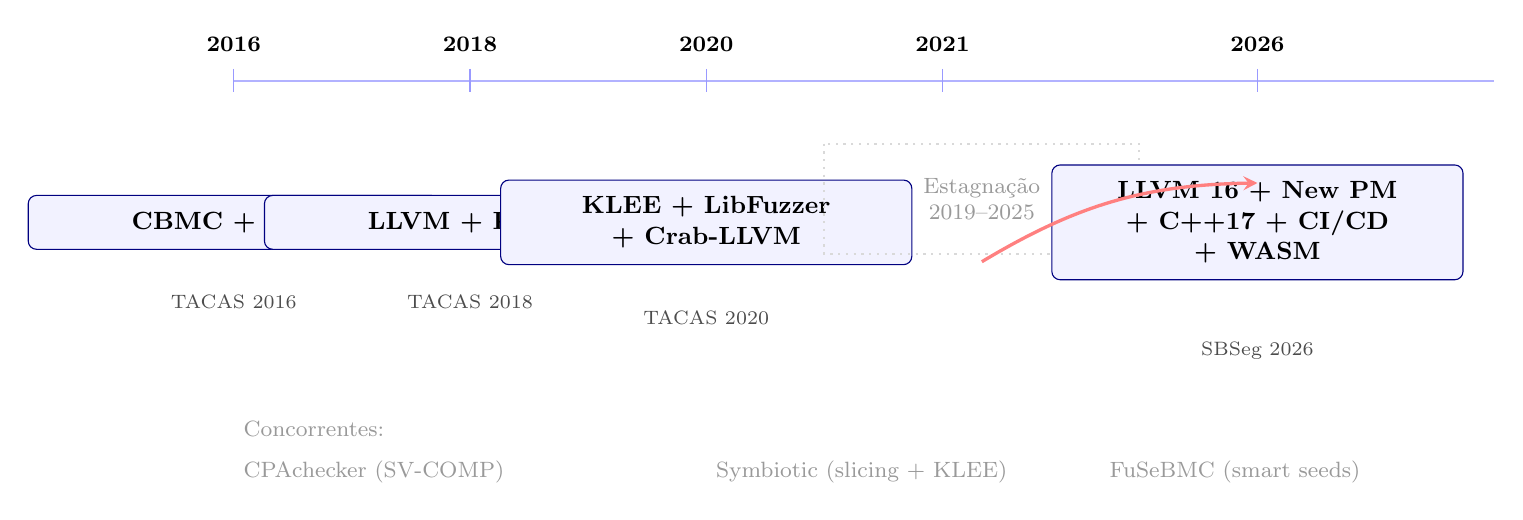
\begin{tikzpicture}[
  node distance=0.2cm,
  year/.style={font=\bfseries\footnotesize, text=black, anchor=south},
  event/.style={align=left, font=\scriptsize, text=black!70, anchor=north},
  milestone/.style={draw=blue!50!black, fill=blue!5, rounded corners=3pt, 
    inner sep=6pt, text width=4.8cm, align=center, font=\small\bfseries},
  rest/.style={font=\footnotesize, text=black!40, align=center},
  arrow/.style={->, >=stealth, thick, blue!40},
]

% Timeline base line
\draw[thick, blue!30] (0,0) -- (16,0);

% Years and tick marks
\foreach \x/\label in {0/2016, 3/2018, 6/2020, 9/2021, 13/2026}{
  \draw[blue!40] (\x,0.15) -- (\x,-0.15);
  \node[year] at (\x,0.25) {\label};
}

% --- 2016 ---
\node[milestone] at (0,-1.8) {CBMC + BMC};
\node[event] at (0,-2.6) {TACAS 2016};

% --- 2018 ---
\node[milestone] at (3,-1.8) {LLVM + KLEE};
\node[event] at (3,-2.6) {TACAS 2018};

% --- 2020 ---
\node[milestone] at (6,-1.8) {KLEE + LibFuzzer\\+ Crab-LLVM};
\node[event] at (6,-2.8) {TACAS 2020};

% --- Stagnation ---
\draw[thick, gray!30, dotted] (7.5,-0.8) rectangle (11.5,-2.2);
\node[rest] at (9.5,-1.5) {Estagnação\\2019--2025};

% --- 2026 ---
\node[milestone] at (13,-1.8) {LLVM 16 + New PM\\+ C++17 + CI/CD\\+ WASM};
\node[event] at (13,-3.2) {SBSeg 2026};

% Concorrentes
\node[rest, anchor=north west] at (0,-4.2) {Concorrentes:};
\node[rest, anchor=north west] at (0,-4.7) {CPAchecker (SV-COMP)};
\node[rest, anchor=north west] at (6,-4.7) {Symbiotic (slicing + KLEE)};
\node[rest, anchor=north west] at (11,-4.7) {FuSeBMC (smart seeds)};

% Renascimento arrow
\draw[->, >=stealth, very thick, red!50] (9.5,-2.3) to[bend left=15] (13,-1.3);

\end{tikzpicture}


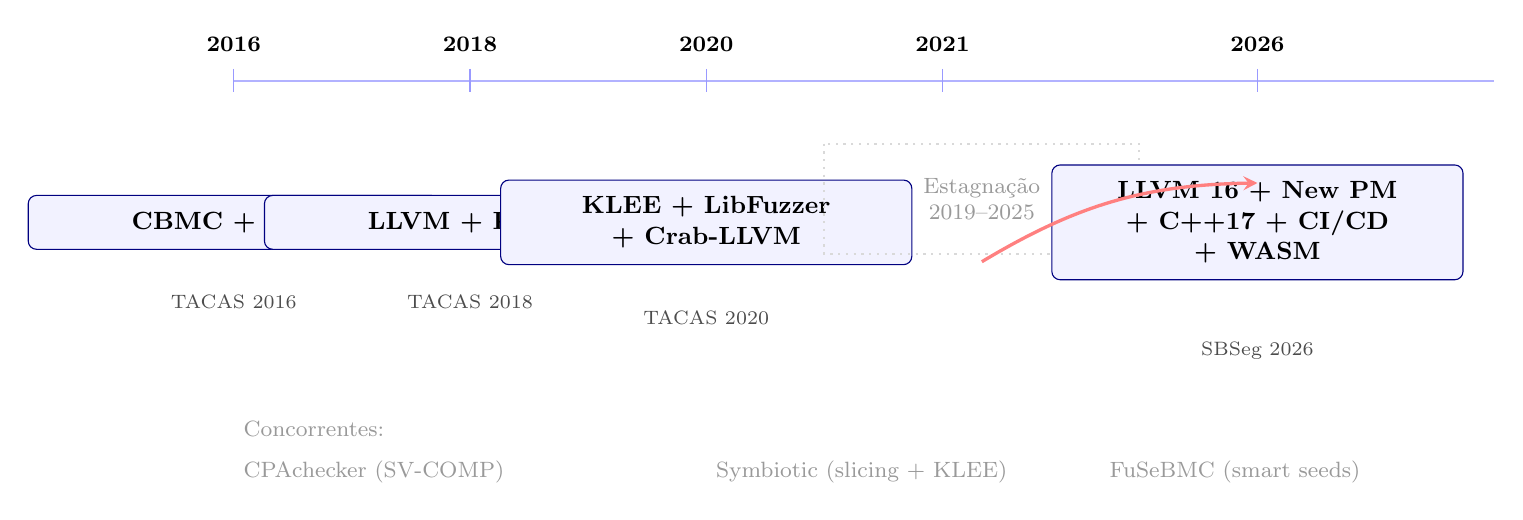
\begin{tikzpicture}[
  node distance=0.2cm,
  year/.style={font=\bfseries\footnotesize, text=black, anchor=south},
  event/.style={align=left, font=\scriptsize, text=black!70, anchor=north},
  milestone/.style={draw=blue!50!black, fill=blue!5, rounded corners=3pt, 
    inner sep=6pt, text width=4.8cm, align=center, font=\small\bfseries},
  rest/.style={font=\footnotesize, text=black!40, align=center},
  arrow/.style={->, >=stealth, thick, blue!40},
]

% Timeline base line
\draw[thick, blue!30] (0,0) -- (16,0);

% Years and tick marks
\foreach \x/\label in {0/2016, 3/2018, 6/2020, 9/2021, 13/2026}{
  \draw[blue!40] (\x,0.15) -- (\x,-0.15);
  \node[year] at (\x,0.25) {\label};
}

% --- 2016 ---
\node[milestone] at (0,-1.8) {CBMC + BMC};
\node[event] at (0,-2.6) {TACAS 2016};

% --- 2018 ---
\node[milestone] at (3,-1.8) {LLVM + KLEE};
\node[event] at (3,-2.6) {TACAS 2018};

% --- 2020 ---
\node[milestone] at (6,-1.8) {KLEE + LibFuzzer\\+ Crab-LLVM};
\node[event] at (6,-2.8) {TACAS 2020};

% --- Stagnation ---
\draw[thick, gray!30, dotted] (7.5,-0.8) rectangle (11.5,-2.2);
\node[rest] at (9.5,-1.5) {Estagnação\\2019--2025};

% --- 2026 ---
\node[milestone] at (13,-1.8) {LLVM 16 + New PM\\+ C++17 + CI/CD\\+ WASM};
\node[event] at (13,-3.2) {SBSeg 2026};

% Concorrentes
\node[rest, anchor=north west] at (0,-4.2) {Concorrentes:};
\node[rest, anchor=north west] at (0,-4.7) {CPAchecker (SV-COMP)};
\node[rest, anchor=north west] at (6,-4.7) {Symbiotic (slicing + KLEE)};
\node[rest, anchor=north west] at (11,-4.7) {FuSeBMC (smart seeds)};

% Renascimento arrow
\draw[->, >=stealth, very thick, red!50] (9.5,-2.3) to[bend left=15] (13,-1.3);

\end{tikzpicture}


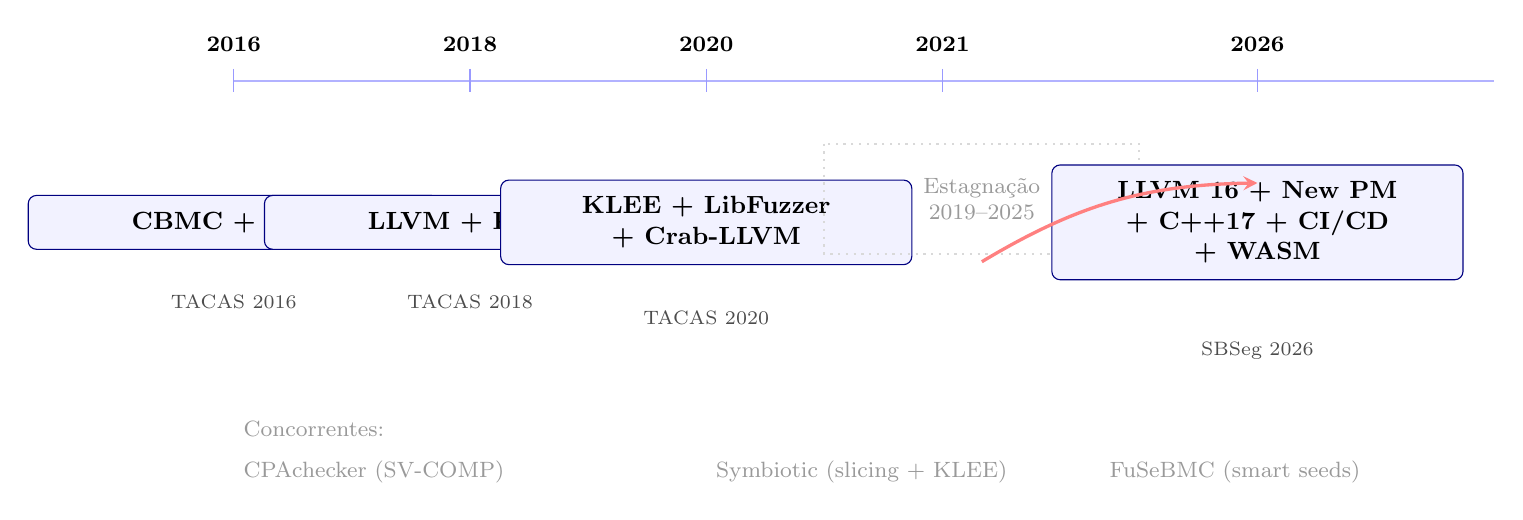
\begin{tikzpicture}[
  node distance=0.2cm,
  year/.style={font=\bfseries\footnotesize, text=black, anchor=south},
  event/.style={align=left, font=\scriptsize, text=black!70, anchor=north},
  milestone/.style={draw=blue!50!black, fill=blue!5, rounded corners=3pt, 
    inner sep=6pt, text width=4.8cm, align=center, font=\small\bfseries},
  rest/.style={font=\footnotesize, text=black!40, align=center},
  arrow/.style={->, >=stealth, thick, blue!40},
]

% Timeline base line
\draw[thick, blue!30] (0,0) -- (16,0);

% Years and tick marks
\foreach \x/\label in {0/2016, 3/2018, 6/2020, 9/2021, 13/2026}{
  \draw[blue!40] (\x,0.15) -- (\x,-0.15);
  \node[year] at (\x,0.25) {\label};
}

% --- 2016 ---
\node[milestone] at (0,-1.8) {CBMC + BMC};
\node[event] at (0,-2.6) {TACAS 2016};

% --- 2018 ---
\node[milestone] at (3,-1.8) {LLVM + KLEE};
\node[event] at (3,-2.6) {TACAS 2018};

% --- 2020 ---
\node[milestone] at (6,-1.8) {KLEE + LibFuzzer\\+ Crab-LLVM};
\node[event] at (6,-2.8) {TACAS 2020};

% --- Stagnation ---
\draw[thick, gray!30, dotted] (7.5,-0.8) rectangle (11.5,-2.2);
\node[rest] at (9.5,-1.5) {Estagnação\\2019--2025};

% --- 2026 ---
\node[milestone] at (13,-1.8) {LLVM 16 + New PM\\+ C++17 + CI/CD\\+ WASM};
\node[event] at (13,-3.2) {SBSeg 2026};

% Concorrentes
\node[rest, anchor=north west] at (0,-4.2) {Concorrentes:};
\node[rest, anchor=north west] at (0,-4.7) {CPAchecker (SV-COMP)};
\node[rest, anchor=north west] at (6,-4.7) {Symbiotic (slicing + KLEE)};
\node[rest, anchor=north west] at (11,-4.7) {FuSeBMC (smart seeds)};

% Renascimento arrow
\draw[->, >=stealth, very thick, red!50] (9.5,-2.3) to[bend left=15] (13,-1.3);

\end{tikzpicture}


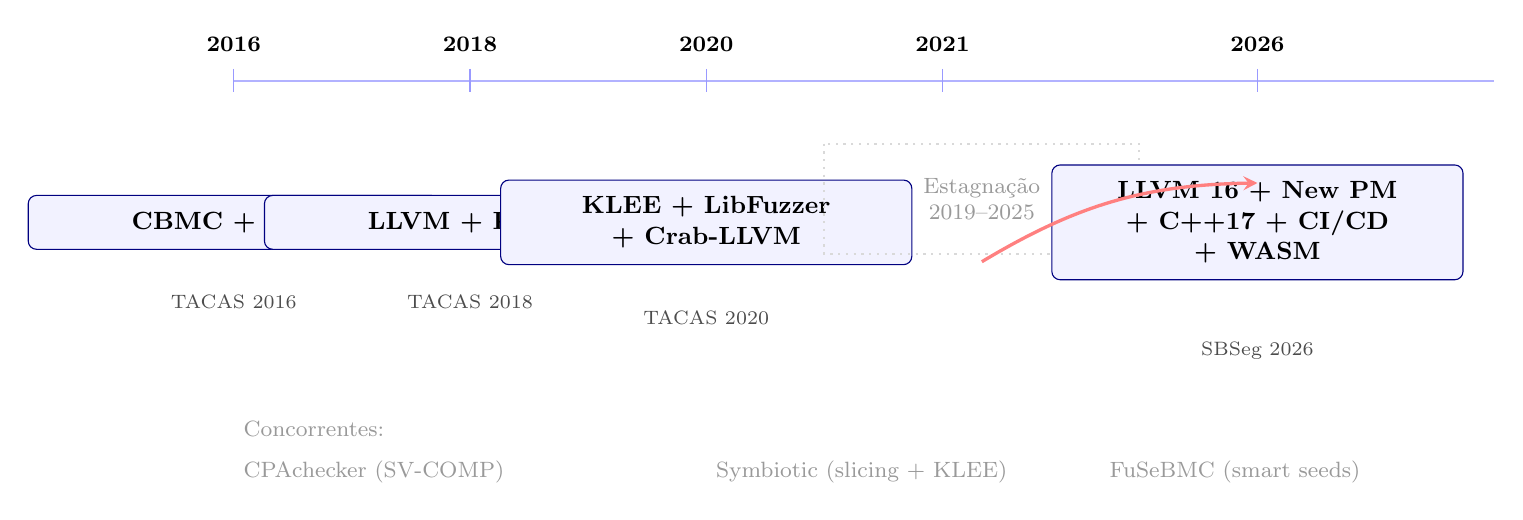
\begin{tikzpicture}[
  node distance=0.2cm,
  year/.style={font=\bfseries\footnotesize, text=black, anchor=south},
  event/.style={align=left, font=\scriptsize, text=black!70, anchor=north},
  milestone/.style={draw=blue!50!black, fill=blue!5, rounded corners=3pt, 
    inner sep=6pt, text width=4.8cm, align=center, font=\small\bfseries},
  rest/.style={font=\footnotesize, text=black!40, align=center},
  arrow/.style={->, >=stealth, thick, blue!40},
]

% Timeline base line
\draw[thick, blue!30] (0,0) -- (16,0);

% Years and tick marks
\foreach \x/\label in {0/2016, 3/2018, 6/2020, 9/2021, 13/2026}{
  \draw[blue!40] (\x,0.15) -- (\x,-0.15);
  \node[year] at (\x,0.25) {\label};
}

% --- 2016 ---
\node[milestone] at (0,-1.8) {CBMC + BMC};
\node[event] at (0,-2.6) {TACAS 2016};

% --- 2018 ---
\node[milestone] at (3,-1.8) {LLVM + KLEE};
\node[event] at (3,-2.6) {TACAS 2018};

% --- 2020 ---
\node[milestone] at (6,-1.8) {KLEE + LibFuzzer\\+ Crab-LLVM};
\node[event] at (6,-2.8) {TACAS 2020};

% --- Stagnation ---
\draw[thick, gray!30, dotted] (7.5,-0.8) rectangle (11.5,-2.2);
\node[rest] at (9.5,-1.5) {Estagnação\\2019--2025};

% --- 2026 ---
\node[milestone] at (13,-1.8) {LLVM 16 + New PM\\+ C++17 + CI/CD\\+ WASM};
\node[event] at (13,-3.2) {SBSeg 2026};

% Concorrentes
\node[rest, anchor=north west] at (0,-4.2) {Concorrentes:};
\node[rest, anchor=north west] at (0,-4.7) {CPAchecker (SV-COMP)};
\node[rest, anchor=north west] at (6,-4.7) {Symbiotic (slicing + KLEE)};
\node[rest, anchor=north west] at (11,-4.7) {FuSeBMC (smart seeds)};

% Renascimento arrow
\draw[->, >=stealth, very thick, red!50] (9.5,-2.3) to[bend left=15] (13,-1.3);

\end{tikzpicture}
